% !TeX spellcheck = pl_PL
\section{System przechowywania danych}
Rozdział ten przedstawia propozycję systemu przechowywania danych. Struktura sieci informatycznej jest rozbudowana, zatem aby scentralizować dostęp do danych zastosowano technologię NAS. 

\subsection{Struktura NAS}
Dostęp do serwera NAS nie wymagają telefony IP oraz bramka VoIP, zatem nie zostały uwzględnione w strukturze. Schemat systemu NAS znajduje się na rysunku \ref{schemat:schemat_sieci_NAS}.
\begin{landscape}
	\hspace{4cm}
	\begin{figure}[!h]
		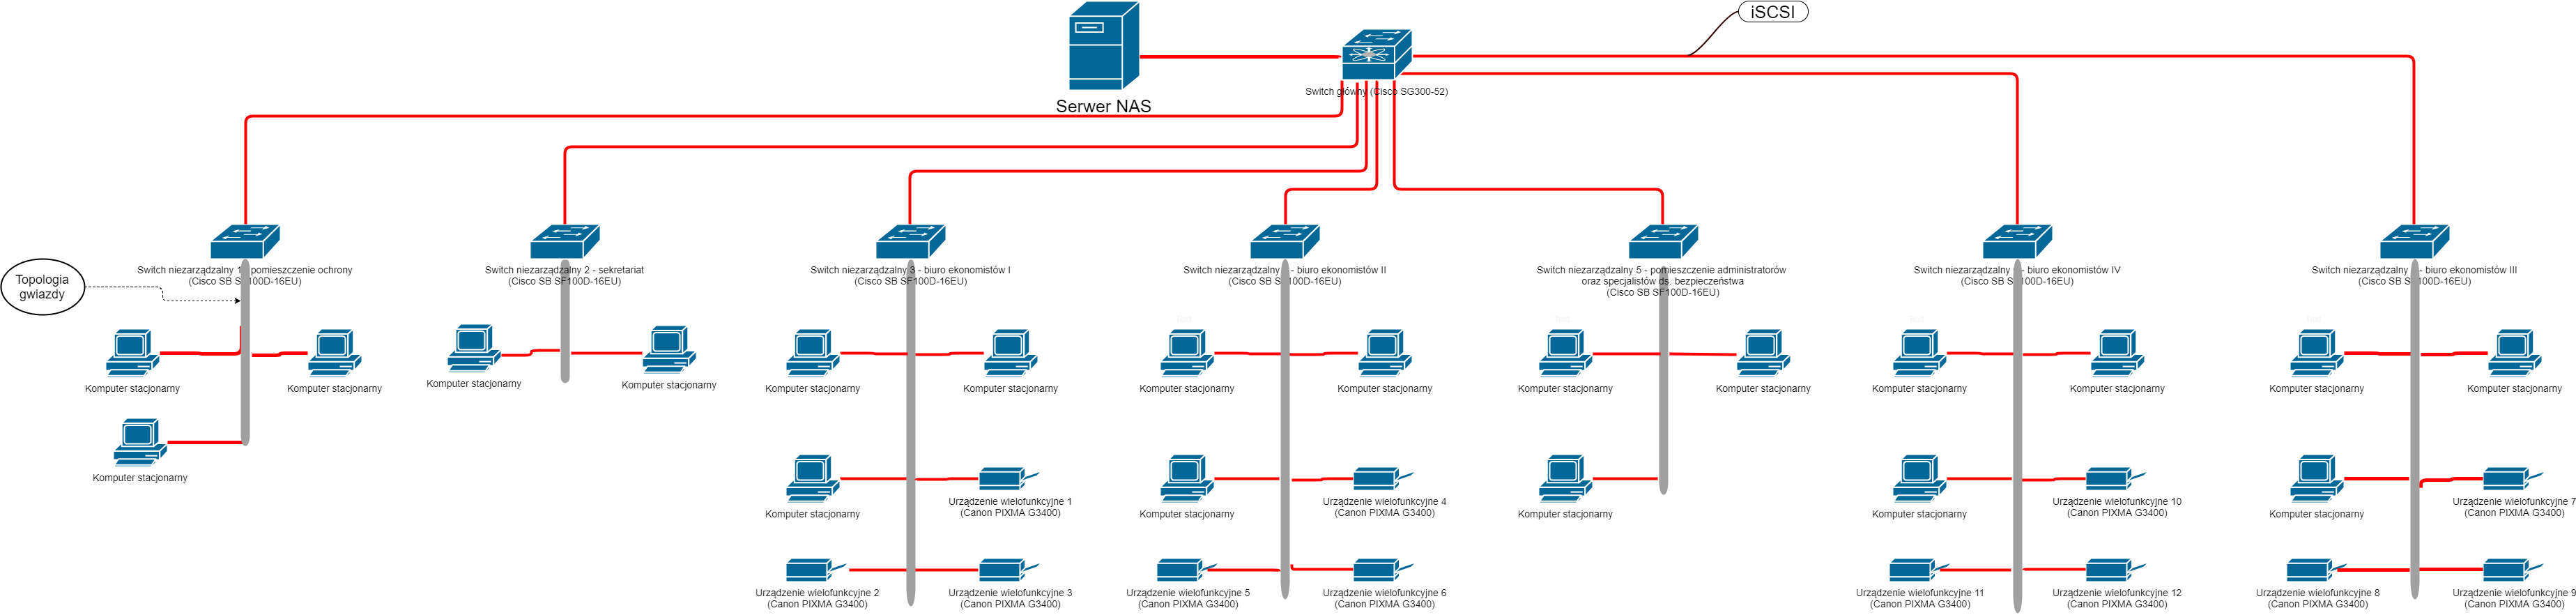
\includegraphics[width=24cm]{Schemat_NAS.png}
		\caption{Schemat struktury NAS}
		\label{schemat:schemat_sieci_NAS}
	\end{figure}
\end{landscape}